\section{データベースの設計}
本システムで使用するデータベースMySQLのテーブルについて示します。また、ERモデルで表したER図式を図\ref{fig:ER}で示します。
\begin{figure}[h]
	\begin{center}
	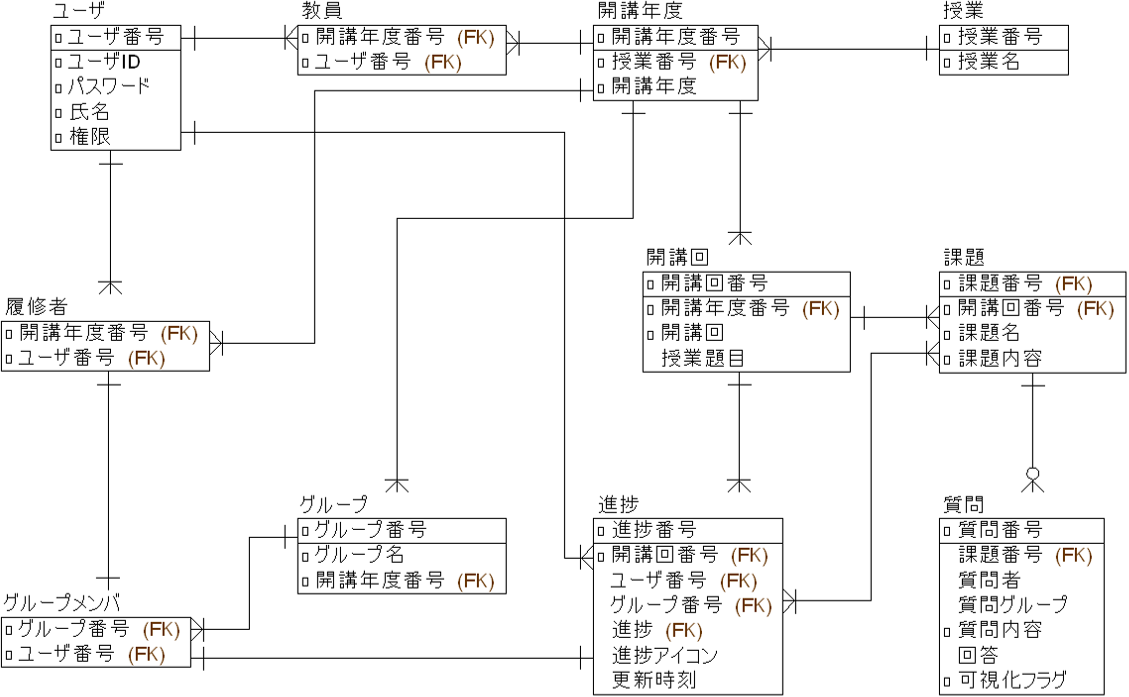
\includegraphics[]{er.png}
	\caption{実体関連図式}
	\label{fig:ER}
	\end{center}
\end{figure}
\subsection{ユーザテーブル}
本システム利用者のユーザ情報を格納します。権限が「学生」であるユーザ情報は、登録日から設定した年が経過すると削除されます。各フィールドの概要は以下の通りです。また、ユーザテーブルの詳細は表\ref{ユーザテーブル}で示します。
\begin{itemize}
	\item ユーザ番号:ユーザテーブルの主キー
	\item ユーザID:システムにおいてユーザを一意に定める名前
	\item パスワード:ユーザの識別・確認に用いるパスワード
	\item 氏名:ユーザ本人の名前
	\item 権限:ユーザに「教員」、「アシスタント」または「学生」のいずれかの権限を与える
\end{itemize}

	\begin{table}[h]
		\centering
		\caption{ユーザテーブル}
		\label{ユーザテーブル}
		\begin{tabular}{|l|l|l|c|l|}
		\hline
		フィールド & 型  & 外部キー & Null & オプション\\ \hline\hline
		{\ul ユーザ番号} & \begin{tabular}[c]{@{}l@{}}INT\\ UNSIGNED\end{tabular} &  & No & AUTO\_INCREMENT\\ \hline
		ユーザID & VARCHAR(32) & & No & UNIQUE\\ \hline
		パスワード & VARCHAR(64) & & No & \\ \hline
		氏名 & VARCHAR(16) &  & No  &\\ \hline
		権限 & ENUM & & No & \\ \hline
		\end{tabular}
	\end{table}
\subsection{グループテーブル}
授業のために作成されたグループ情報を格納します。各フィールドの概要は以下の通りです。また、グループテーブルの詳細は表\ref{グループテーブル}で示します。
\begin{itemize}
	\item グループ番号:グループテーブルの主キー
	\item グループ名:グループの名前
	\item 開講年度番号:何年度の何の授業のために作成されたかを示す
\end{itemize}

	\begin{table}[h]
		\centering
		\caption{グループテーブル}
		\label{グループテーブル}
		\begin{tabular}{|l|l|l|c|l|}
		\hline
		フィールド & 型 & 外部キー & Null & オプション\\ \hline\hline
		{\ul グループ番号} & \begin{tabular}[c]{@{}l@{}}INT\\ UNSIGNED\end{tabular} & & No & AUTO\_INCREMENT \\ \hline
		グループ名 & VARCHAR(16) & & No & \\ \hline
		開講年度番号 & \begin{tabular}[c]{@{}l@{}}INT\\ UNSIGNED\end{tabular} & 授業 & No & \\ \hline
		\end{tabular}
	\end{table}
\subsection{グループメンバテーブル}
授業のために作成されたグループに所属しているユーザ情報を格納します。各フィールドの概要は以下の通りです。また、グループメンバテーブルの詳細は表\ref{グループメンバテーブル}で示します。
\begin{itemize}
	\item グループ番号:何年度の何の授業のために作成されたグループであるかを示す
	\item メンバ:グループに所属している学生
\end{itemize}

	\begin{table}[h]
		\centering
		\caption{グループメンバテーブル}
		\label{グループメンバテーブル}
		\begin{tabular}{|l|l|l|c|l|}
		\hline
		フィールド & 型 & 外部キー & Null & オプション\\ \hline\hline
		グループ番号 & \begin{tabular}[c]{@{}l@{}}INT\\ UNSIGNED\end{tabular} & グループ & No & \\ \hline
		メンバ & \begin{tabular}[c]{@{}l@{}}INT\\ UNSIGNED\end{tabular} & ユーザ & No & \\ \hline
		\end{tabular}
	\end{table}
\subsection{授業テーブル}
本システムを利用する授業の情報を格納します。各フィールドの概要は以下の通りです。また、授業テーブルの詳細は表\ref{授業テーブル}で示します。
\begin{itemize}
	\item 授業番号:授業テーブルの主キー
	\item 授業名:授業の名前
\end{itemize}

	\begin{table}[h]
		\centering
		\caption{授業テーブル}
		\label{授業テーブル}
		\begin{tabular}{|l|l|l|c|l|}
		\hline
		フィールド & 型 & 外部キー & Null & オプション \\ \hline\hline
		{\ul 授業番号} & \begin{tabular}[c]{@{}l@{}}INT\\ UNSIGNED\end{tabular} & & No & AUTO\_INCREMENT \\ \hline
		授業名 & VARCHAR(32) & & No & UNIQUE \\ \hline
		\end{tabular}
	\end{table}
\subsection{開講年度テーブル}
開講された年度を含めた授業情報を格納します。各フィールドの概要は以下の通りです。また、開講年度テーブルの詳細は表\ref{開講年度テーブル}で示します。
\begin{itemize}
	\item 開講年度番号:開講年度テーブルの主キー
	\item 授業番号:授業を示す
	\item 開講年度:開講された年度を示す
\end{itemize}

	\begin{table}[h]
		\centering
		\caption{開講年度テーブル}
		\label{開講年度テーブル}
		\begin{tabular}{|l|l|l|c|l|}
		\hline
		フィールド & 型 & 外部キー & Null & オプション \\ \hline\hline
		{\ul 開講年度番号} & \begin{tabular}[c]{@{}l@{}}INT\\ UNSIGNED\end{tabular} & & No & AUTO\_INCREMENT \\ \hline
		授業番号 & \begin{tabular}[c]{@{}l@{}}INT\\ UNSIGNED\end{tabular} & 授業 & No & \\ \hline
		開講年度 & \begin{tabular}[c]{@{}l@{}}SMALLINT\\ UNSIGNED\end{tabular} & & No & \\ \hline
		\end{tabular}
	\end{table}
\subsection{開講回テーブル}
回ごとの授業情報を格納します。各フィールドの概要は以下の通りです。また、開講回テーブルの詳細は表\ref{開講回テーブル}で示します。
\begin{itemize}
	\item 開講回番号:開講回テーブルの主キー
	\item 開講年度番号:何年度の何の授業であるかを示す
	\item 開講回:何年度の何の授業の何回目に開講されたかを示す
	\item 授業題目:開講された回ごとの授業概要を示す
\end{itemize}

	\begin{table}[h]
		\centering
		\caption{開講回テーブル}
		\label{開講回テーブル}
		\begin{tabular}{|l|l|l|c|l|}
		\hline
		フィールド & 型 & 外部キー & Null & オプション \\ \hline\hline
		{\ul 開講回番号} & \begin{tabular}[c]{@{}l@{}}INT\\ UNSIGNED\end{tabular} &  & No & AUTO\_INCREMENT \\ \hline
		開講年度番号    & \begin{tabular}[c]{@{}l@{}}INT\\ UNSIGNED\end{tabular} & 授業開講年度 & No & \\ \hline
		開講回 & \begin{tabular}[c]{@{}l@{}}TINYINT\\ UNSIGNED\end{tabular} & & No & \\ \hline
		授業題目 & VARCHAR(256) & & & \\ \hline
		\end{tabular}
	\end{table}
\subsection{教員テーブル}
授業を担当するユーザ情報を格納します。各フィールドの概要は以下の通りです。また、教員テーブルの詳細は表\ref{教員テーブル}で示します。
\begin{itemize}
	\item 開講年度番号:何年度の何の授業であるかを示す
	\item 講師番号:授業を担当する教員およびアシスタントユーザ
\end{itemize}

	\begin{table}[h]
		\centering
		\caption{教員テーブル}
		\label{教員テーブル}
		\begin{tabular}{|l|l|l|c|l|}
		\hline
		フィールド & 型 & 外部キー & Null & オプション \\ \hline\hline
		開講年度番号 & \begin{tabular}[c]{@{}l@{}}INT\\ UNSIGNED\end{tabular} & 授業開講年度 & No & \\ \hline
		講師番号 & \begin{tabular}[c]{@{}l@{}}INT\\ UNSIGNED\end{tabular} & ユーザ & No & \\ \hline
		\end{tabular}
	\end{table}
\subsection{履修者テーブル}
受講するユーザ情報を格納します。各フィールドの概要は以下の通りです。また、履修者テーブルの詳細は表\ref{履修者テーブル}で示します。
\begin{itemize}
	\item 開講年度番号:何年度の何の授業であるかを示す
	\item 履修者番号:授業を履修する学生ユーザ
\end{itemize}

	\begin{table}[h]
		\centering
		\caption{履修者テーブル}
		\label{履修者テーブル}
		\begin{tabular}{|l|l|l|c|l|}
		\hline
		フィールド & 型 & 外部キー & Null & オプション \\ \hline\hline
		開講年度番号 & \begin{tabular}[c]{@{}l@{}}INT\\ UNSIGNED\end{tabular} & 授業開講年度 & No & \\ \hline
		履修者番号 & \begin{tabular}[c]{@{}l@{}}INT\\ UNSIGNED\end{tabular} & ユーザ & No & \\ \hline
		\end{tabular}
	\end{table}
\subsection{課題テーブル}
授業の回ごとに提示する課題情報を格納します。各フィールドの概要は以下の通りです。また、課題テーブルの詳細は表\ref{課題テーブル}で示します。
\begin{itemize}
	\item 課題番号:課題テーブルの主キー
	\item 開講回番号:何年度の何の授業の何回目の授業であるかを示す
	\item 課題名:授業回ごとに提示される課題の番号
	\item 課題内容:授業回ごとに提示される課題の内容
\end{itemize}

	\begin{table}[h]
		\centering
		\caption{課題テーブル}
		\label{課題テーブル}
		\begin{tabular}{|l|l|l|c|l|}
		\hline
		フィールド & 型 & 外部キー & Null & オプション \\ \hline\hline
		{\ul 課題番号} & \begin{tabular}[c]{@{}l@{}}INT\\ UNSIGNED\end{tabular} & & No & AUTO\_INCREMENT \\ \hline
		開講回番号 & \begin{tabular}[c]{@{}l@{}}INT\\ UNSIGNED\end{tabular} & 開講回 & No & \\ \hline
		課題名 & VARCHAR(8) & & No  & \\ \hline
		課題内容 & VARCHAR(512) & & No & \\ \hline
		\end{tabular}
	\end{table}
\subsection{進捗テーブル}
授業回ごとの学生の課題の進捗情報を格納します。進捗情報は授業時間内のみで使用するため、授業終了から一定期間後に格納された情報は削除されます。各フィールドの概要は以下の通りです。また、進捗テーブルの詳細は表\ref{進捗テーブル}で示します。
\begin{itemize}
	\item 進捗番号:進捗テーブルの主キー
	\item 開講回番号:何年度の何の授業の何回目の授業であるかを示す
	\item ユーザ番号:進捗を確認する対象である受講者
	\item グループ番号:進捗を確認する対象である受講グループ
	\item 進捗:進捗の最終更新時刻の時点までに達成している課題
	\item 進捗アイコン:進捗確認画面で表示されるアイコンの種類
	\item 更新時刻:進捗の最終更新時刻
\end{itemize}

	\begin{table}[h]
		\centering
		\caption{進捗テーブル}
		\label{進捗テーブル}
		\begin{tabular}{|l|l|l|c|l|}
		\hline
		フィールド & 型 & 外部キー & Null & オプション \\ \hline\hline
		{\ul 進捗番号} & \begin{tabular}[c]{@{}l@{}}INT\\ UNSIGNED\end{tabular} & & No & AUTO\_INCREMENT \\ \hline
		開講回番号 & \begin{tabular}[c]{@{}l@{}}INT\\ UNSIGNED\end{tabular} & 開講回 & No & \\ \hline
		ユーザ番号 & \begin{tabular}[c]{@{}l@{}}INT\\ UNSIGNED\end{tabular} & ユーザ  & & \\ \hline
		グループ番号 & \begin{tabular}[c]{@{}l@{}}INT\\ UNSIGNED\end{tabular} & グループ & & \\ \hline
		進捗 & \begin{tabular}[c]{@{}l@{}}INT\\ UNSIGNED\end{tabular} & 課題 & & \\ \hline
		進捗アイコン & ENUM & & & \\ \hline
		更新時刻 & TIME & & & \\ \hline
		\end{tabular}
	\end{table}
\subsection{質問テーブル}
授業回ごとに出た質問の情報を格納します。各フィールドの概要は以下の通りです。また、質問テーブルの詳細は表\ref{質問テーブル}で示します。
\begin{itemize}
	\item 質問番号:質問テーブルの主キー
	\item 質問者:質問をした学生
	\item 質問グループ:質問をしたグループ
	\item 質問内容:課題に対する質問の内容
	\item 回答:質問に対する回答
	\item 可視化フラグ:過去に出た質問の中で、学生に質問や回答を表示させるかどうかのフラグ
\end{itemize}

	\begin{table}[h]
		\centering
		\caption{質問テーブル}
		\label{質問テーブル}
		\begin{tabular}{|l|l|l|c|l|}
		\hline
		フィールド & 型 & 外部キー & Null & オプション \\ \hline\hline
		{\ul 質問番号} & \begin{tabular}[c]{@{}l@{}}INT\\ UNSIGNED\end{tabular} & & No & AUTO\_INCREMENT \\ \hline
		課題番号 & \begin{tabular}[c]{@{}l@{}}INT\\ UNSIGNED\end{tabular} & 課題 &  & \\ \hline
		質問者 & VARCHAR(16) & & & \\ \hline
		質問グループ & VARCHAR(16) & & & \\ \hline
		質問内容 & VARCHAR(512) & & No & \\ \hline
		回答 & VARCHAR(512) & & & \\ \hline
		可視化フラグ & BOOLEAN &  & No & DEFAULT TRUE\\ \hline
		\end{tabular}
	\end{table}